\documentclass[border=8pt]{standalone}
\usepackage{amsmath,amssymb}
\usepackage{tikz}
\usetikzlibrary{arrows.meta,backgrounds}
\begin{document}
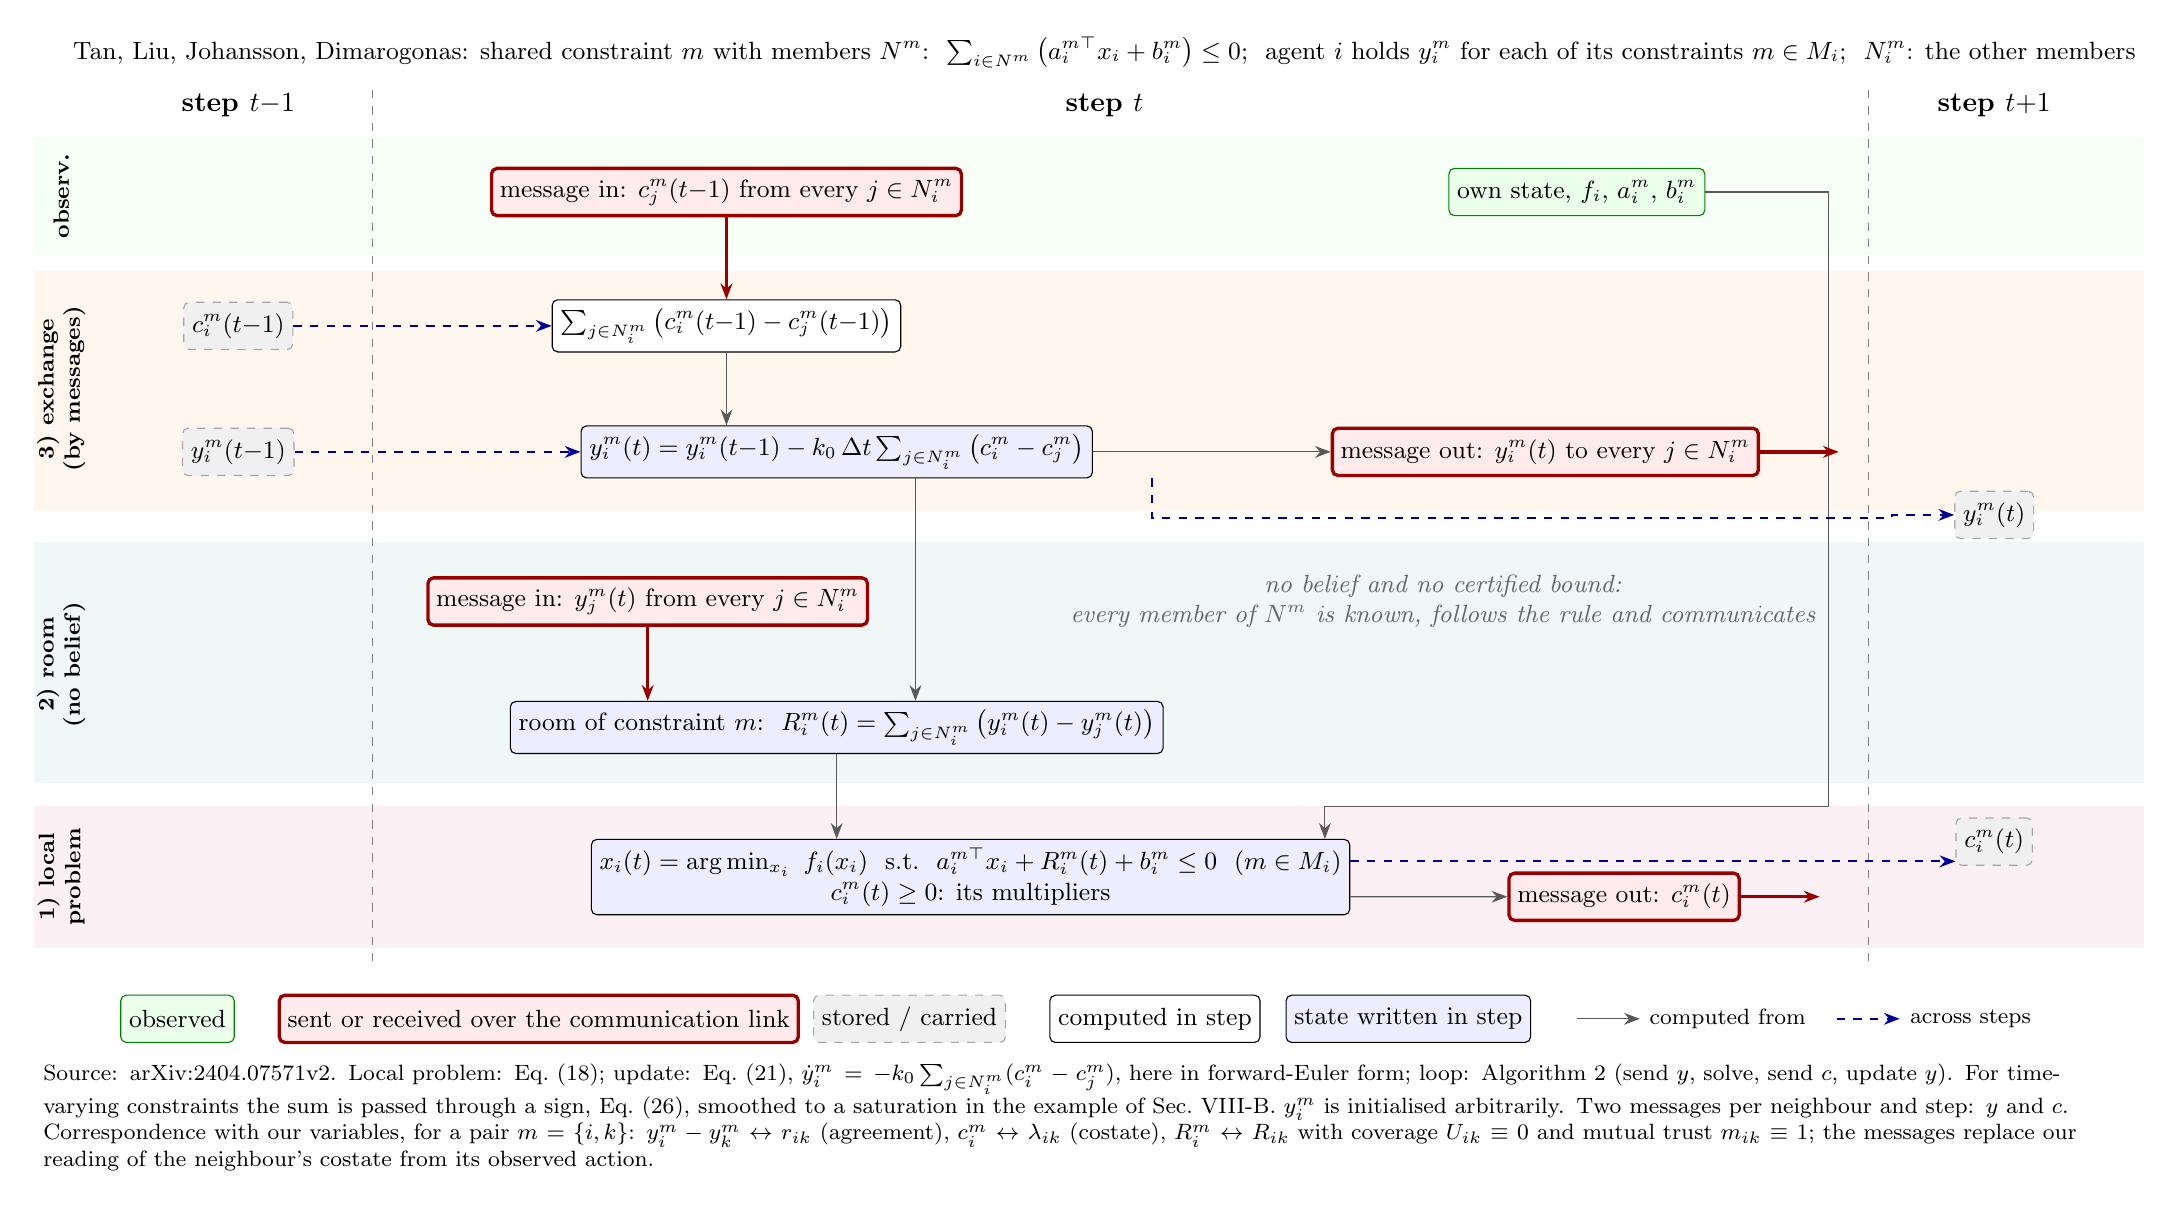
\begin{tikzpicture}[x=1cm,y=1cm,font=\small,>={Stealth[length=2mm]},
  obs/.style={draw=green!50!black,fill=green!8,rounded corners=2pt,inner sep=3pt,minimum height=6mm},
  msg/.style={draw=red!60!black,fill=red!8,rounded corners=2pt,inner sep=3pt,minimum height=6mm,very thick},
  sto/.style={draw=gray!70,fill=gray!12,dashed,rounded corners=2pt,inner sep=3pt,minimum height=6mm},
  cmp/.style={draw=black,fill=white,rounded corners=2pt,inner sep=3pt,minimum height=6mm},
  st/.style={cmp,fill=blue!7},
  e/.style={->,draw=black!65},
  ms/.style={->,draw=red!60!black,very thick},
  carry/.style={->,draw=blue!60!black,dashed,thick}]
\def\yO{0}\def\yS{-1.7}\def\yX{-3.3}\def\yB{-5.2}\def\yR{-6.8}\def\yQ{-8.7}
\def\xa{0}\def\xb{22.3}
\begin{scope}[on background layer]
\fill[green!4] (-2.6,\yO+0.7) rectangle (24.2,\yO-0.8);
\fill[orange!7] (-2.6,\yS+0.7) rectangle (24.2,\yX-0.75);
\fill[teal!6] (-2.6,\yB+0.75) rectangle (24.2,\yR-0.7);
\fill[purple!6] (-2.6,\yQ+0.9) rectangle (24.2,\yQ-0.9);
\draw[gray,dashed] (1.7,1.3)--(1.7,-9.8); \draw[gray,dashed] (20.7,1.3)--(20.7,-9.8);
\end{scope}
\node[font=\bfseries] at (\xa,1.1) {step $t{-}1$};
\node[font=\bfseries] at (11,1.1) {step $t$};
\node[font=\bfseries] at (\xb,1.1) {step $t{+}1$};
\node[font=\small,anchor=south] at (11,1.45) {Tan, Liu, Johansson, Dimarogonas: shared constraint $m$ with members $N^m$:\ \ $\sum_{i\in N^m}\big(a_i^{m\top}x_i+b_i^m\big)\le0$;\ \ agent $i$ holds $y_i^m$ for each of its constraints $m\in M_i$;\ \ $N_i^m$: the other members};
\node[rotate=90,font=\bfseries\footnotesize] at (-2.25,-0.05) {observ.};
\node[rotate=90,font=\bfseries\footnotesize,align=center] at (-2.25,-2.5) {3) exchange\\(by messages)};
\node[rotate=90,font=\bfseries\footnotesize,align=center] at (-2.25,-6.0) {2) room\\(no belief)};
\node[rotate=90,font=\bfseries\footnotesize,align=center] at (-2.25,\yQ) {1) local\\problem};

\node[sto] (cP) at (\xa,\yS) {$c_i^m(t{-}1)$};
\node[sto] (yP) at (\xa,\yX) {$y_i^m(t{-}1)$};

\node[obs] (own) at (17.0,\yO) {own state, $f_i$, $a_i^m$, $b_i^m$};
\node[msg] (cin) at (6.2,\yO) {message in: $c_j^m(t{-}1)$ from every $j\in N_i^m$};
\node[cmp] (imb) at (6.2,\yS) {$\sum_{j\in N_i^m}\big(c_i^m(t{-}1)-c_j^m(t{-}1)\big)$};
\node[st] (y) at (7.6,\yX) {$y_i^m(t)=y_i^m(t{-}1)-k_0\,\Delta t\sum_{j\in N_i^m}\big(c_i^m-c_j^m\big)$};
\node[msg] (yout) at (16.6,\yX) {message out: $y_i^m(t)$ to every $j\in N_i^m$};
\node[msg] (yin) at (5.2,\yB) {message in: $y_j^m(t)$ from every $j\in N_i^m$};
\node[font=\small\itshape,text=black!60,align=center] at (15.3,\yB) {no belief and no certified bound:\\ every member of $N^m$ is known, follows the rule and communicates};
\node[st] (R) at (7.6,\yR) {room of constraint $m$:\ \ $R_i^m(t)=\sum_{j\in N_i^m}\big(y_i^m(t)-y_j^m(t)\big)$};
\node[st,align=center] (qp) at (9.3,\yQ) {$x_i(t)=\arg\min_{x_i}\ f_i(x_i)$\ \ s.t.\ \ $a_i^{m\top}x_i+R_i^m(t)+b_i^m\le0\ \ (m\in M_i)$\\ $c_i^m(t)\ge0$: its multipliers};
\node[msg] (cout) at (17.6,\yQ-0.25) {message out: $c_i^m(t)$};

\node[sto] (yN) at (\xb,\yX-0.8) {$y_i^m(t)$};
\node[sto] (cN) at (\xb,\yQ+0.45) {$c_i^m(t)$};

\draw[ms] (cin)--(imb); \draw[e] (imb.south)--(imb.south |- y.north);
\draw[e] (y)--(yout);
\draw[e] ([xshift=10mm]y.south)--([xshift=10mm]y.south |- R.north);
\draw[ms] (yin.south)--(yin.south |- R.north);
\draw[e] (R.south)--(R.south |- qp.north);
\draw[e] (own.east)-|(20.2,\yQ+0.9)-|([xshift=45mm]qp.north);
\draw[e] ([yshift=-2.5mm]qp.east)--(cout.west);
\draw[carry] (cP.east)--(imb.west);
\draw[carry] (yP.east)--(yP.east -| y.west);
\draw[carry] ([xshift=40mm]y.south)--++(0,-0.5)-|(21.0,\yX-0.8)--(yN.west);
\draw[carry] ([yshift=2mm]qp.east)--([yshift=2mm]qp.east -| cN.west);
\draw[ms] (yout.east)--++(1.0,0) node[right,font=\footnotesize,text=red!60!black] {};
\draw[ms] (cout.east)--++(1.0,0);

\node[obs,anchor=west] (L1) at (-1.5,-10.5) {observed};
\node[msg,anchor=west] (L0) at (0.5,-10.5) {sent or received over the communication link};
\node[sto,anchor=west] (L2) at (7.3,-10.5) {stored / carried};
\node[cmp,anchor=west] (L3) at (10.3,-10.5) {computed in step};
\node[st,anchor=west] (L4) at (13.3,-10.5) {state written in step};
\draw[e] (17.0,-10.5)--(17.8,-10.5) node[right,font=\footnotesize] {computed from};
\draw[carry] (20.3,-10.5)--(21.1,-10.5) node[right,font=\footnotesize] {across steps};
\node[anchor=north west,font=\footnotesize,align=left,text width=26cm] at (-2.6,-10.95) {Source: arXiv:2404.07571v2. Local problem: Eq.~(18); update: Eq.~(21), $\dot y_i^m=-k_0\sum_{j\in N_i^m}(c_i^m-c_j^m)$, here in forward-Euler form; loop: Algorithm~2 (send $y$, solve, send $c$, update $y$). For time-varying constraints the sum is passed through a sign, Eq.~(26), smoothed to a saturation in the example of Sec.~VIII-B. $y_i^m$ is initialised arbitrarily. Two messages per neighbour and step: $y$ and $c$.\\ Correspondence with our variables, for a pair $m=\{i,k\}$: $y_i^m-y_k^m\leftrightarrow r_{ik}$ (agreement), $c_i^m\leftrightarrow\lambda_{ik}$ (costate), $R_i^m\leftrightarrow R_{ik}$ with coverage $U_{ik}\equiv0$ and mutual trust $m_{ik}\equiv1$; the messages replace our reading of the neighbour's costate from its observed action.};
\end{tikzpicture}
\end{document}
